\documentclass[11pt]{article}
\usepackage{graphicx} % Required for inserting images
\usepackage[top=2.5cm, bottom=2.5cm, left=2cm, right=2cm]{geometry}
\usepackage[T1]{fontenc}
\usepackage{wrapfig}
\usepackage{hyperref}
\usepackage[utf8]{inputenc}
\usepackage{multirow}
\usepackage{subcaption}
\usepackage{booktabs}
\usepackage{bookmark}
\usepackage{graphicx}
\usepackage{setspace}
\setlength{\parindent}{0in}
\usepackage{physics}
\usepackage{tikz}
\usepackage{tikz-3dplot}
\usepackage[outline]{contour} % glow around text
\usepackage{xcolor}
\usepackage{float}
\usepackage{makeidx}
\usepackage{fancyhdr}
\usepackage{pgfplots}
\usepackage{amsmath}
\pgfplotsset{compat=1.18}
\usepackage{caption}
\usepackage[english,catalan]{babel}
\setlength{\parskip}{11pt}
\usepackage{xcolor}
\usepackage{listings}
\usepackage{marginnote}
\usepackage{siunitx}
\usepackage{framed}
\usepackage{ulem}


\title{\Huge\bfseries Pràctica 6: \\ Feixos de raigs catòdics \\ [2ex] \Large}

\author{\begin{tabular}{c}
\textbf{GRUP A6} \\
Isaac Baldi García (1667260)\\
Miguel Ordejón de Prada (1710966) \\
Eira Jacas García (1666616) \\
Víctor Bosch González (1676373)
\end{tabular}}

\date{Març 2025}

\begin{document}

\maketitle
\begin{center}
    \textbf{Abstract: En aquesta pràctica s'estudia el comportament d'un feix de raigs catòdics sota un camp elèctirc i un camp magnètic amb l'objectiu de determinar propietats de les partícules que els conformen. Concretament, analitzant les desviacions del feix dels raigs sota aquests camps s'obté la relació entre la càrrega i la massa d'aquestes particules.} 
\end{center}


\newpage

\tableofcontents
\newpage

\section{Introducció teòrica}\label{sec: intro}

En l'experiment tenim un condensador de plaques plano-paral·leles que són finites en la direcció $Y$ i infinites en la direcció $Z$. Anomenem $l$ a la llargada de les plaques (cap a la direcció $Y$), $L$ una altura arbitrària (cap a la direcció $Z$) i $d$ la distància de separació entre les plaques.
\begin{equation}
    \frac{Q}{L} \approx \varepsilon \sum_i E_i \, \Delta l_i \approx \varepsilon \sum_i \frac{\Delta V_i \, \Delta l_i}{\Delta r_i}
    \label{eq: Q}
\end{equation}
on $\frac{Q }{L }$ és la càrrega per unitat de longitud del condensador, $\varepsilon$ la peritivitat del medi dielèctric, $\Delta V_i$, $\Delta l_i$ i $\Delta r_i$ les diferències de voltatge entre les plaques, distància tangencial i distància radial corresponentment.

Per calcular la capacitat ideal d'un condensador de plaques plano-paral·lels com el que tenim a l'experiment calculem la diferència de potencial entre les plaques 
\begin{equation}
    |\Delta\phi|=\int_{0}^{d} \vec{E}\vec{dl}= Ed
\end{equation}
i com que assumim que el camp és uniforme i de valor $\frac{\sigma}{\varepsilon}$\footnote{És molt fàcil obtenir aquest resultat sumant el camp de dos plans infinits de càrrega oposada que s'obté amb la llei de Gauss} podem obtenir la capacitat per per unitat de longitud de la següent manera
\begin{equation}
    \Delta\phi=Ed=\frac{\sigma d}{\varepsilon}
    =Q\frac{d}{lL\varepsilon}=\frac{Q}{C}\implies (\frac{C}{L})_t=\frac{l\varepsilon}{d}
    \label{eq: c_t}
\end{equation}
\section{Mètode experimental i simulacions}\label{sec: metode}
\subsection{Part experimental}
-hem dividit la corba de pot en 20 segments...

\subsection{tractament de dades exp i simulacions}
Per calc el camp hem calculat el vector perp a la recta entre dos punts exp adjacents.

\section{Resultats i discussió}\label{sec: resultats}
En aquesta secció presentem i comparem els resultats obtinguts tant experimental com computacionalment. Mostrem les línies de camp i les línies equipotencials de tres distribucions de càrrega així com el resultat experimental de la capacitat d'una d'elles. Per fer les simulacions hem solucionat l'equació de Laplace amb el mètode de Jacobi\footnote{Codi i breu descripció a l'annex \ref{sec: annex}}. Cal destacar que les simulacions les hem fet al buit, ja que no coneixem el valor de la permetivitat del dielèctric. A més, s'ha considerat que els elèctrodes són conductors ideals i constitueixen les úniques fonts del camp.

\subsection{Condensador de plaques plano-paral·leles}\label{sec: cond}
La primera distribució de càrrega que estudiarem és un condensador de plaques plano-paral·leles centrat a l'orígen. Les plaques són paral·leles al pla $XZ$, finites en la direcció $Y$ i molt llargues o infinies en la direcció $Z$.
En les Figs. (\ref{fig: cond_pot}) i (\ref{fig: cond_e}) podem veure representades les línies de camp elèctric i les línies equipotencials obtingudes tant experimentalment com en la simulació.   
\begin{figure}[h]
    \centering
    \begin{subfigure}{0.495\textwidth}
        \centering
        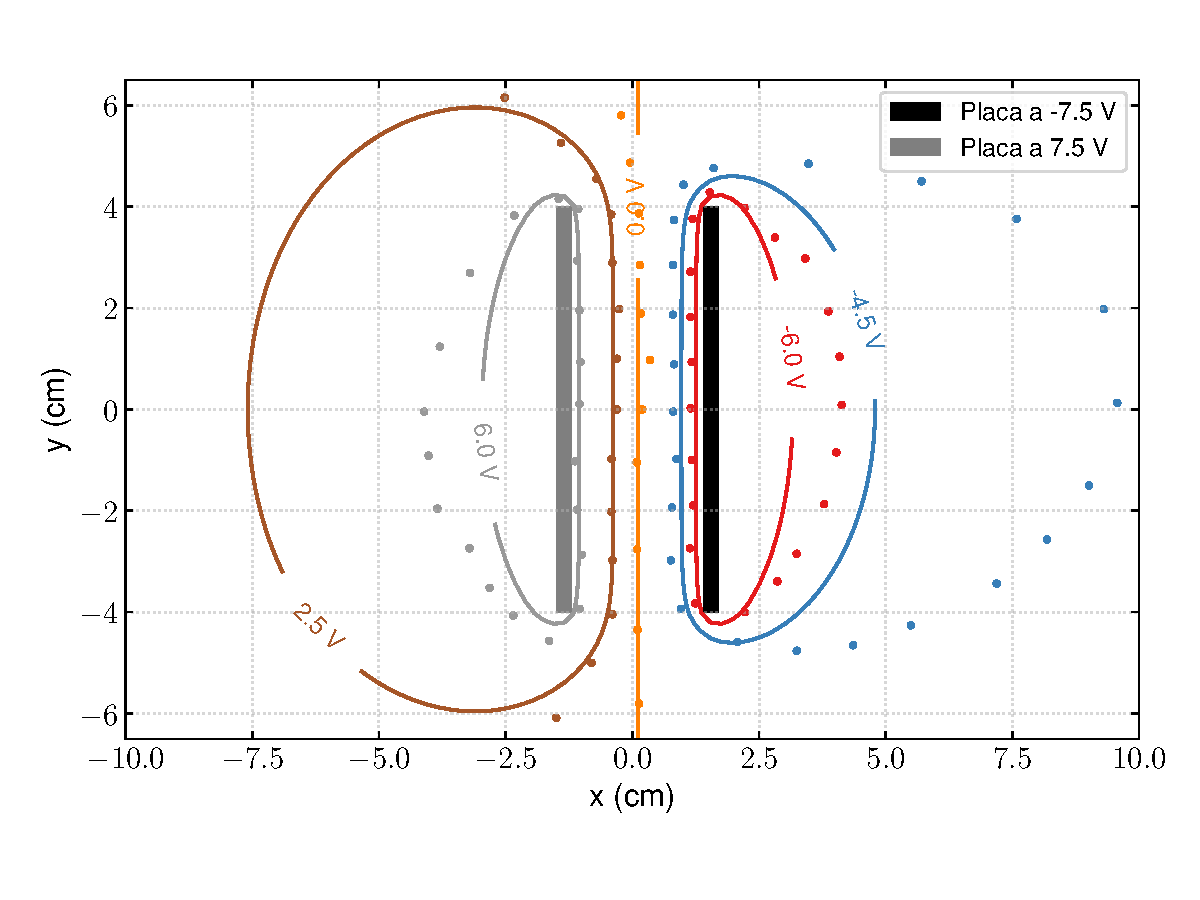
\includegraphics[width=\textwidth]{cond_combi_def.pdf}
        \caption{Línies equipotencials d'un condensador plano-paral·lel. Punts experimentals i línies de la simulació.}
        \label{fig: cond_pot}
    \end{subfigure}
    \begin{subfigure}{0.495\textwidth} 
        \centering
        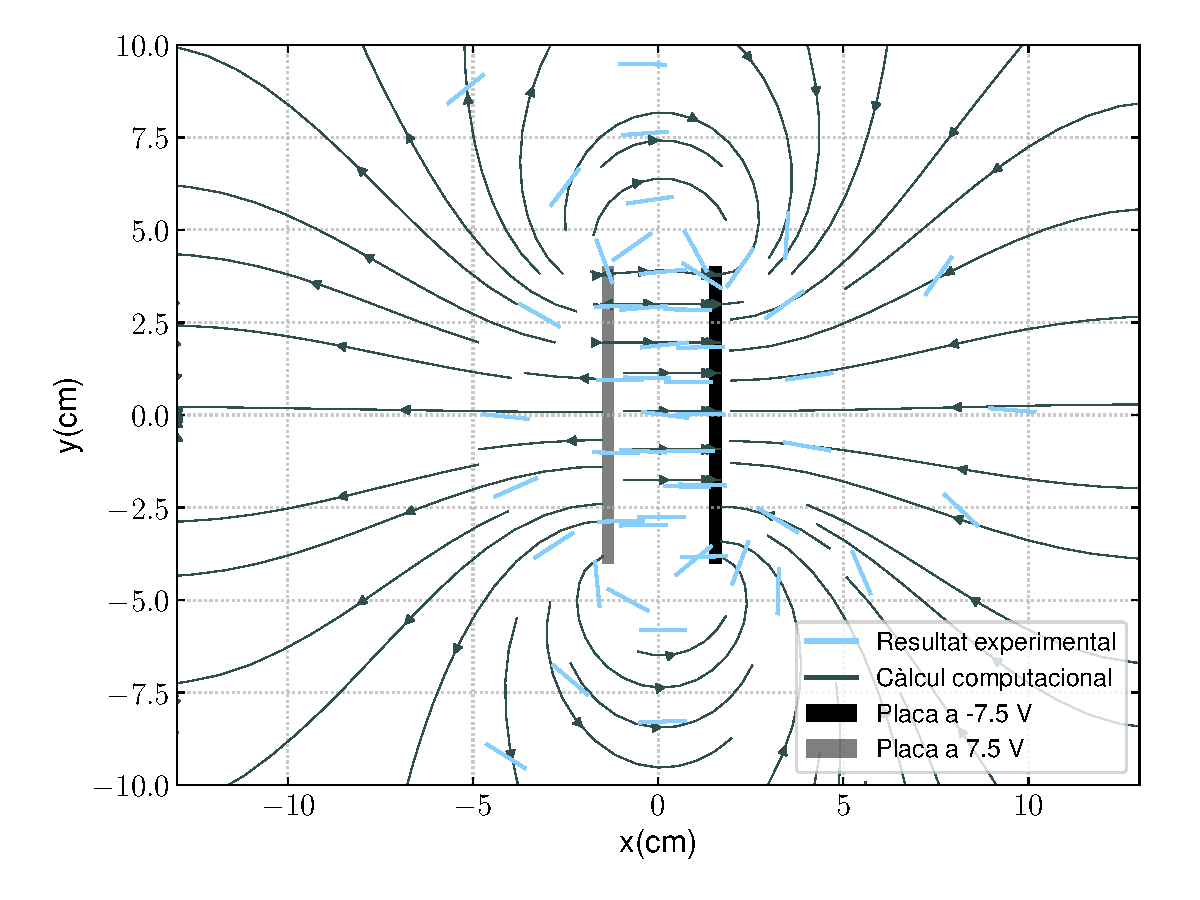
\includegraphics[width=\textwidth]{cond_camp.pdf}
        \caption{Línies de camp elèctric d'un condensador plano-paral·lel. Segments experimentals i línies de la simulació.}
        \label{fig: cond_e}
    \end{subfigure}
\end{figure}

A la Fig. (\ref{fig: cond_pot}) podem veure com a la regió central del condensador les línies equipotencials són paral·leles a les plaques, com prediu la teoria. En canvi, a prop de les vores, les línies es corben fins que s'acaben tancant a causa de la disminució de la component $X$ del camp elèctric. Aquest resultat difereix del cas ideal, (condensador de plaques infinites) en el que les línies equipotencials mai es tanquen. Tanmateix, veiem que coinsideix amb la simulació, on les línies també es tanquen tot i que ho fan més a prop. Aquesta discrepància entre la simulació i l'experiment principalment és a causa de que la simulació està feta al buit i no té en compte la permetivitat relativa del medi. Això genera que el camp simulat sigui més intens i per tant, les línies equipotensials es tanquin més a prop de l'elèctrode. També hi ha altres efectes com les irregularitats dels elèctrodes, la connexió entre la font i els elèctrodes o la discontinuïtat del camp elèctric als límits del paper que no hem tingut en compte a la simulació i poden contribuir a la diferència de resultats.

Pel que fa a la Fig. (\ref{fig: cond_e}) veiem com les línies de camp van des de la placa positiva a la negativa i tenen major densitat a prop d'aquestes, indicant un camp més intens. Com en el cas del potencial, les línies segueixen un comportament semblant al ideal a la part central i, en canvi, a prop de les vores es desvien a causa dels efectes de vorada. Similarment, els segments experimentals que representen la direcció del camp també segueixen la tendència del càlcul computacional tot i que les línies experimentals tendeixen a tancar-se més sobre els electrodes. Aquestes diferències s'expliquen igual que les discutides anteriorment.

Per calcular la capacitat del condensador, primer hem calculat la càrrega per unitat de superfície del condensador en funció de $\varepsilon$, a partir de l'Eq. (\ref{eq: Q}). Tot seguit amb l'Eq () hem calculat la capacitat per unitat de longitud del condensador\footnote{Les dades necessaries per fer els càlculs es poden trobar a la Taula \ref{tab:mesures} de l'annex com també les Eqs. (\ref{eq: ins_q}) i (\ref{eq: ins_c}) pel càlcul d'incerteses.}.

\[
\frac{Q}{L} = \varepsilon  (37{,}65 \pm 9{,}48)\, \mathrm{C/m} \implies
\boxed{ \frac{C}{L} = \varepsilon  (2{,}51 \pm 0{,}63)\, \mathrm{F/m} }
\]    

Aquest resultat el podem comparar amb el resultat tèoric de la capacitat d'un condensador ideal amb les mateixes dimensions. Usant l'Eq. (\ref{eq: c_t}) obtenim $(\frac{C}{L})_t =(2,667 \pm 0,095)\, \mathrm{F/m}$ que és compatible amb el resultat experimental del nostre condensador no ideal.

\subsection{Fils infinits}\label{sec: fils}
La segona configuració són dos fils infinits paral·lels amb càrrega oposada. Conseqüentment, en aquest cas, la simulació representa el cas ideal.
\begin{figure}[h]
    \centering
    \begin{subfigure}{0.495\textwidth}
        \centering
        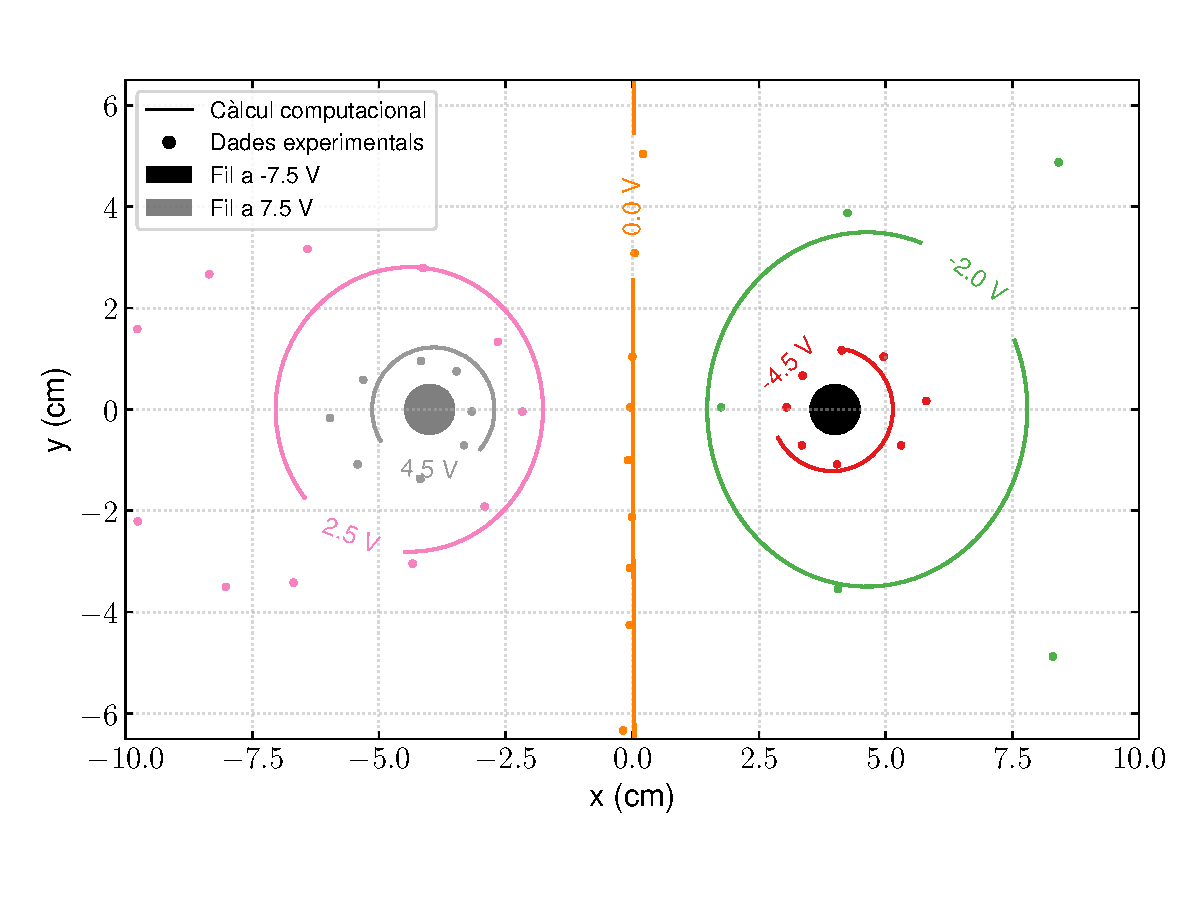
\includegraphics[width=\textwidth]{fils_combi.pdf}
        \caption{Línies equipotencials de dos fils infinits paral·lels i a potencials oposats.}
        \label{fig: fils_pot}
    \end{subfigure}
    \begin{subfigure}{0.495\textwidth} 
        \centering
        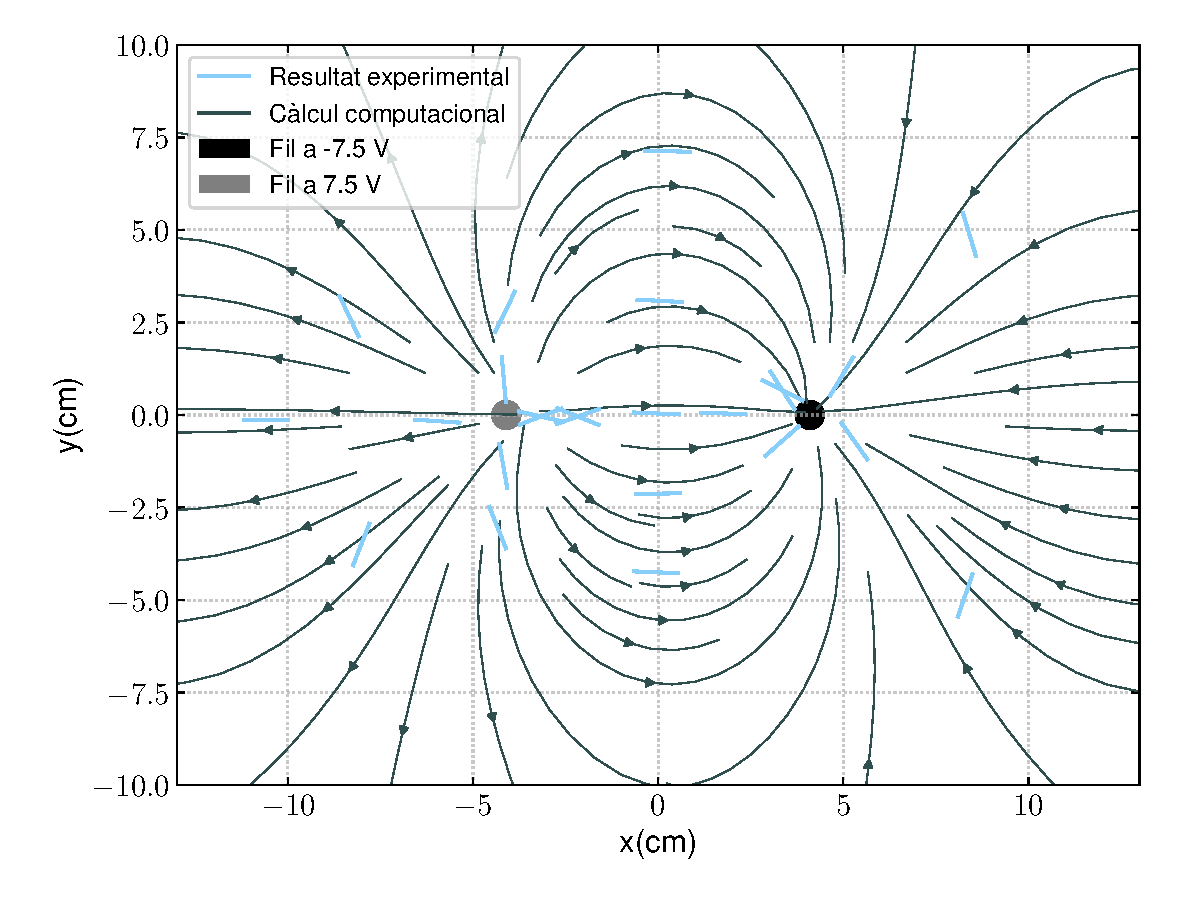
\includegraphics[width=\textwidth]{fils_camp.pdf}
        \caption{Línies de camp elèctric de dos fils infinits paral·lels i a potencials oposats. Segments experimentals i línies de la simulació.}
        \label{fig: fils_camp}
    \end{subfigure}
\end{figure}


A la Fig. \ref{fig: fils_pot} si ens fixem en les línies equipotencials experimentals veiem que es tanquen en el·lipses al voltant dels fils i presenten una assímptota just entre els dos elèctrodes. Aquesta és la tendència dictada per la simulació tot i que en la simulació les línies es tanquen en circumferències. Aquesta diferència pot ser deguda a diversos factors. En primer lloc, el nostre muntatge experimental és una aproximació en dues dimensions del sistema en tres dimensions que intentem replicar. En segon lloc, el nostre sistema té una discontinuïtat del camp elèctric als límits del paper que no hem introduït a la simulació. A més, a la simulació tampoc hem tingut en compte que el medi és dielèctric amb permitivitat diferent a $\epsilon_0$. Per últim, pot haver altres contribuicions al camp que no hem tingut en compte com la unió entre els elèctrodes i la font de corrent o un camp extern present al laboratori.

Veiem com el camp elèctric  experimental mostrat a la Fig. (\ref{fig: fils_camp}) també segueix la tendència de la simulació tot i que les línies de camp que surten del fil a $7.5$ V tenen més tendència a tancar-se cap al fil a $-7.5$ V. Això pot ser degut a que hi ha diversos efectes que no hem tingut en compte a la simulació com hem explicat en el cas del potencial. 

\subsection{Placa amb escletxa i fil infinit}\label{sec:lliure}
La tercera configuració és un fil infinit enfront una placa infinita en l'eix $Z$ amb una escletxa al llarg de la placa i al davant del fil. A més, existeix una diferència de potencialentre el fil i les dues parts de la placa, que sí que estan al mateix potencial. Aquesta, és una disposició similar a la d'un experiment de difracció si tractem el fil com un "emisor" de línies equipotencials i les plaques amb l'escletxa com l'objecte que les difracta. Per tant, la motivació per estudiar aquesta configuració prové de voler veure si amb les línies de potencial passava algun fenòmen similar a la difracció d'ones\footnote{Més informació sobre la difració d'ones a \url{https://en.wikipedia.org/wiki/Diffraction}}.

\begin{figure}[h]
    \centering
    \begin{subfigure}{0.495\textwidth}
        \centering
        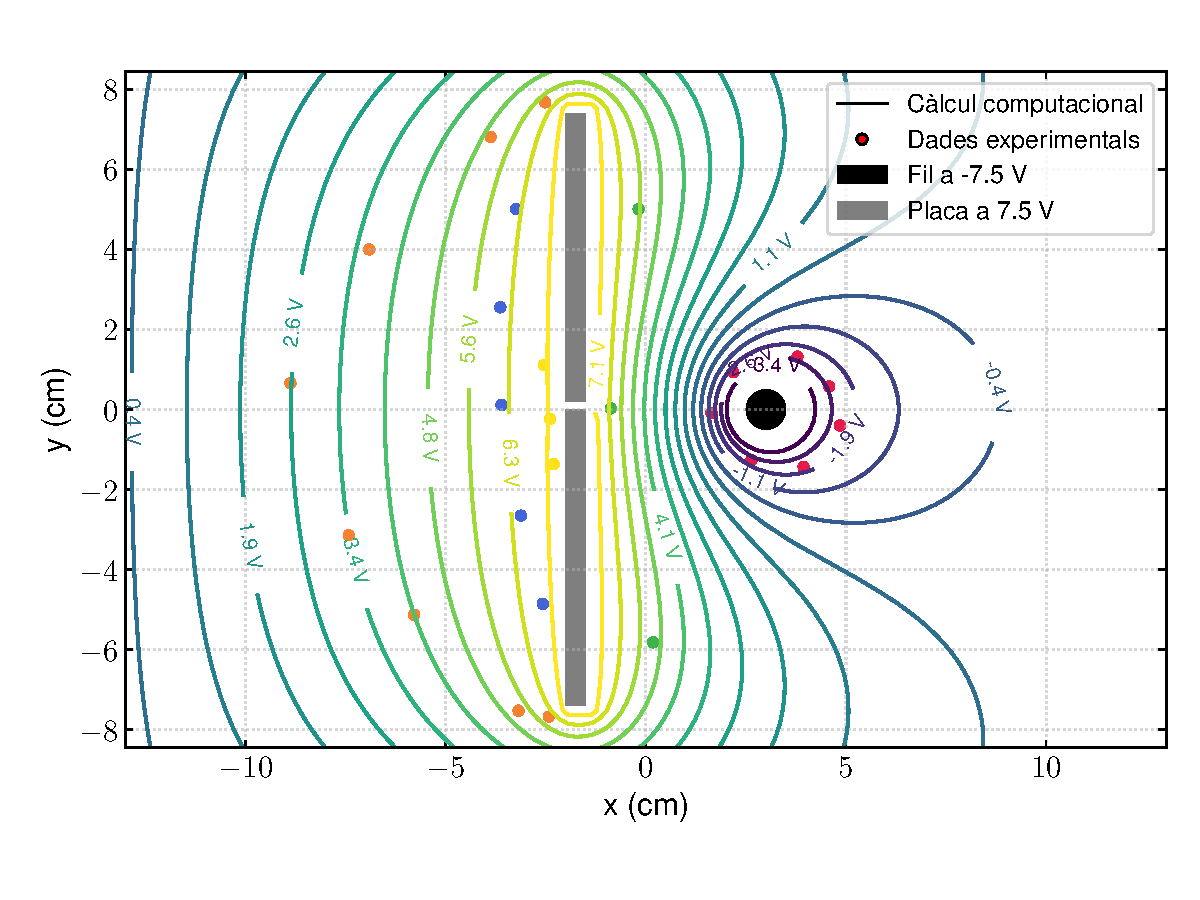
\includegraphics[width=\textwidth]{lliure_combi_e_colors.pdf}
        \caption{Línies equipotencials d'una placa infinita AMB escletxa davant d'un fil infinit. Punts experimentals de color diferent per cada valor de potencial.}
        \label{fig: lliure_pot_e}
    \end{subfigure}
    \begin{subfigure}{0.495\textwidth} 
        \centering
        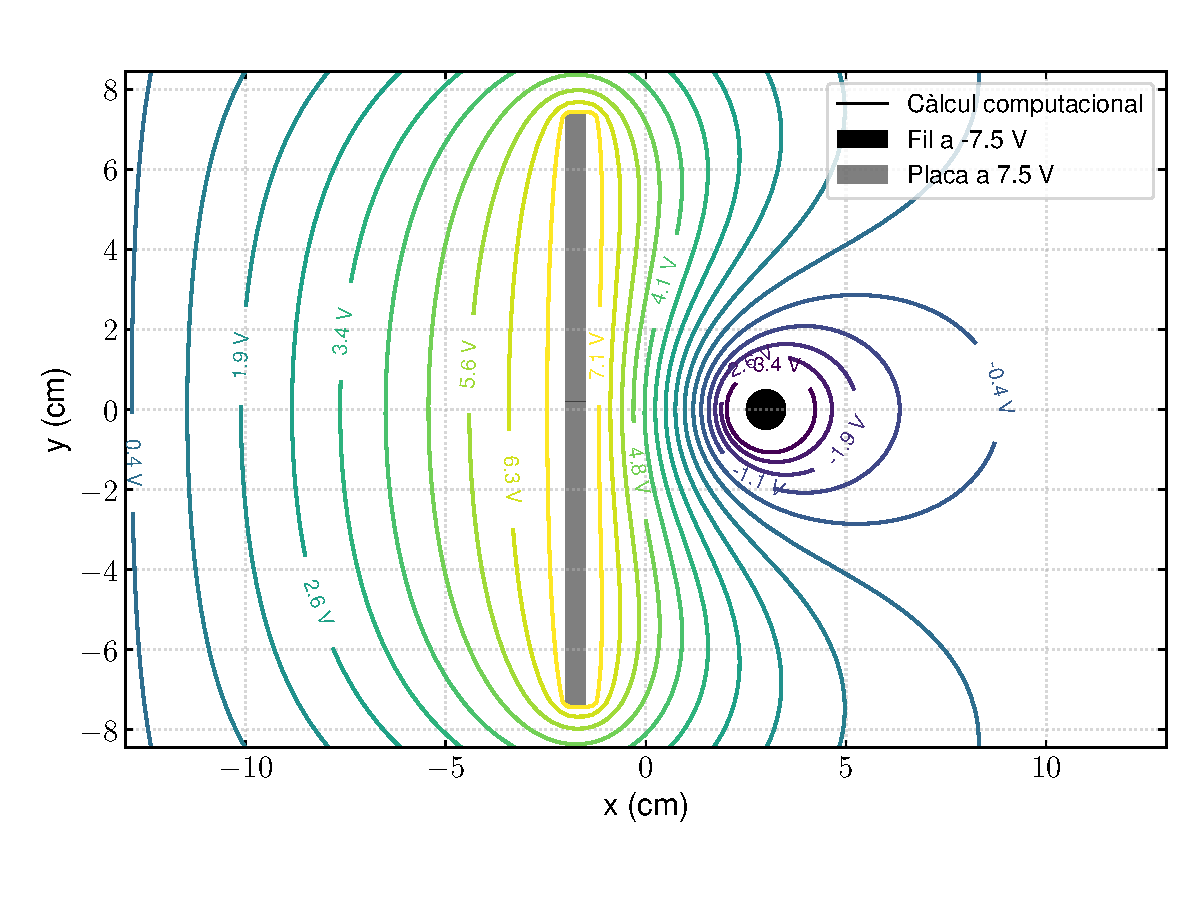
\includegraphics[width=\textwidth]{lliure_combi_0.pdf}
        \caption{Línies equipotencials d'una placa infinita SENSE escletxa davant d'un fil infinit.}
        \label{fig: lliure_pot_0}
    \end{subfigure}
\end{figure}
Si ens fixem en les línies equipotencials experimentals de la Fig. (\ref{fig: lliure_pot_e}) veiem que es comporten de la següent manera: el radi de corbatura de les línies equipotencials va augmentnt a mesura que ens allunyem de l'"emisor" (fil) i ens apropem a l'escletxa, tal com ho faria el front d'ona d'una ona. A l'altre banda de l'escletxa, el radi de corbatura disminueix respecte l'observat abans de l'escletxa de tal forma que és com si l'escletxa fos un segon emisor. Per tant, amb aquesta informació sembla que hi hagi hagut un fenòment de difracció degut a l'escletxa.
No obstant això, si ens fixem en les línies equipotencials simulades veiem clarament que el motiu de la forma de les línies equipotencials no té res a veure amb l'escletxa. El veritable fet que explica les línies equipotencials mostrades és la superposició del potencial elèctric generat pel fil i la placa (que ja en coneixem la forma gràcies a les configuracions anteriors). De fet, com podem veure a la Fig. (\ref{fig: lliure_pot_0})l'existència de l'escletxa quasi bé no afecta a la forma de les línies equipotencials, ja que és molt petita en comparació amb les dimencions del fil i de la placa. Per tant, la difracció no serveix per explicar les observacions experimentals, tot i que, experimentalment, en un principi ho pugui semblar. Aquest resultat, era d'esperar ja que el potencial d'un sistema electroestàtic no depen del temps i, per tant, no pot tenir propietats ondulatòries.
\begin{figure}
    \centering
    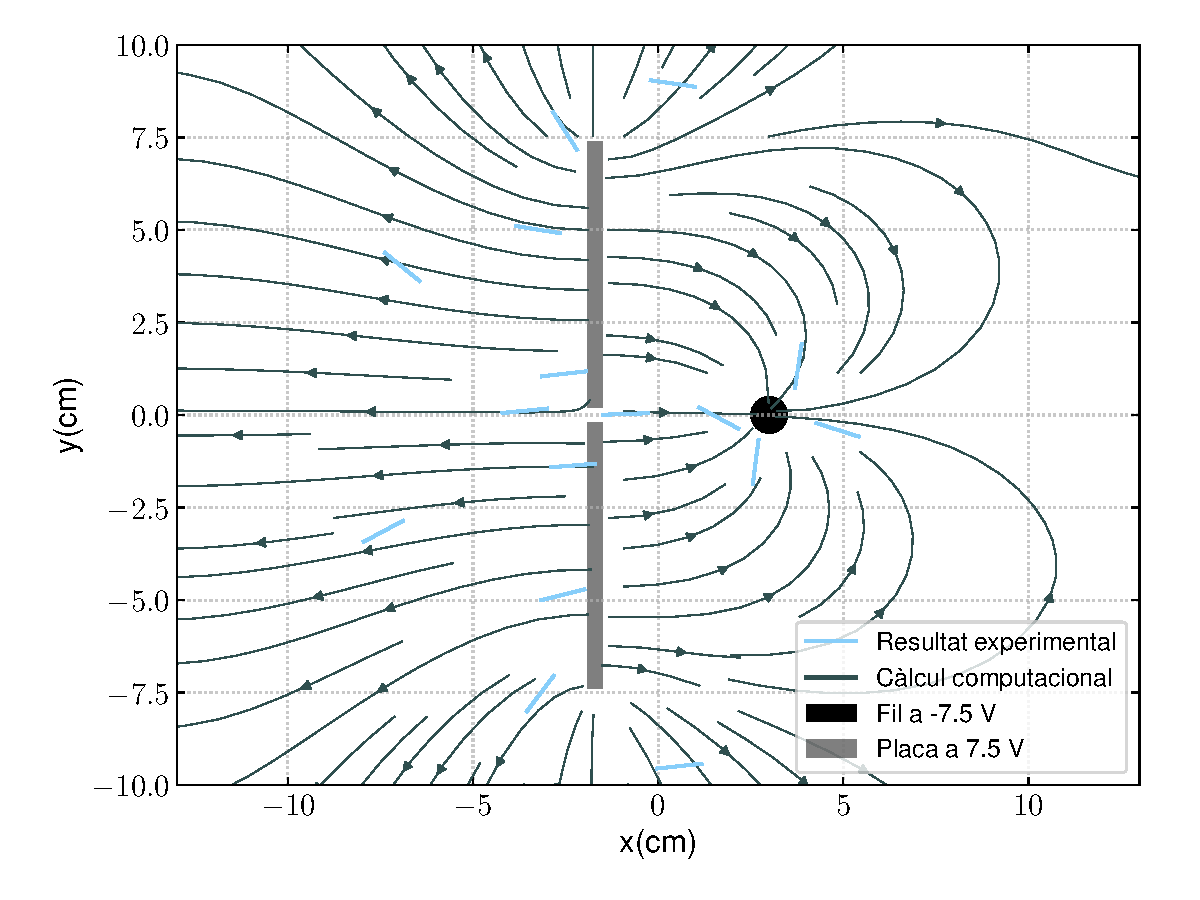
\includegraphics[width=0.45\textwidth]{lliure_camp.pdf}
    \caption{Línies de camp elèctric. Segments experimentals i línies de la simulació.}
    \label{fig: lliure_camp}
\end{figure}

Per altra banda, a la Fig. (\ref{fig: lliure_camp}) podem veure el camp elèctric generat per aquesta configuració. Com en les altres configuracions veiem que el camp experimental seguexi la tendència de la simulació però es tanca més al voltant de les vores de les plaques i dels fils infinits. Aquestes diferències s'expliquen pels mateixos raonaments que en els casos anteriors.


\subsection{Estimació de la permitivitat relativa}
En la secció \ref{sec: cond} hem vist com les línies equipotencials simulades diferien de les experimentals principalment a causa de que la simulació està feta al buit, i en canvi, l'experiment emula un dielèctric. Aprofitarem aquestes diferencies per estimar el valor de la permitivitat relativa d'aquest dielèctric, $\varepsilon_r$.

En el cas ideal, dins del conductor, el camp elèctric queda fixat per la distància entre plaques, $d$, i la diferència de potencial $V$. Fora del condensador, però, el camp sí que depèn d'$\varepsilon_r$. 
Assumint que podem expressar el potencial al buit com 
\begin{equation}
    \phi_0 = \frac{U}{\varepsilon_0}
\end{equation} 
on $U$ és una funció desconeguda\footnote{Això sempre ho podem fer perquè podem expressar el nostre sistema com la suma de moltes càrregues puntuals}.Llavors el potencial en el dielèctric (l.i.h.) serà
\begin{equation}
    \phi(r)=\frac{\phi_0(r)}{\varepsilon_r}.
    \label{eq: epsilon}
\end{equation} 
Per poder treballar còmodament posem el 0 de potencial a una de les dues plaques i per calcular $\varepsilon_r$ només hem d'evaluar l'Eq. (\ref{eq: epsilon}) a diferents punts. Agafant diferents punts experimentals i evaluant-ne el potencial teòric al buit trobem el valor de $\varepsilon_r$. Fent la mitjana entre els valors obtinguts hem estimat\footnote{Càlcul d'inserteses a l'annex}
\begin{equation}
    \varepsilon_r=(1,98 \pm 0,10)\, \mathrm{F/m}
\end{equation}

\section{Conclusions}\label{sec: conc}

En aquesta pràctica hem estudiat les línies equipotencials i de camp dins d'un material dielèctric de tres configuracions de conductors diferents gràcies al paral·lelisme entre les equacions del camp de corrents i del camp de desplaçament. 

En primer lloc hem estudiat un condensador de plaques plano-paral·leles finites en una dimensió i hem pogut veure com les línies de camp es tancaven al voltant de les plàque a diferència del cas ideal. També hem vist com la simulació al buit coïncidia en tendència amb l'experiment però les línies equipotencials simulades es tancaven més aprop de les plaques a causa de que el camp elèctric al buit és més intens. A més, hem realitzat un càlcul experimental de la capacitat del condensador i hem obtingut un valor de $ \frac{C}{L} = \varepsilon  (2{,}51 \pm 0{,}63)\, \mathrm{F/m} $ que es compatible amb resultat del model ideal.

En segon lloc hem estudiat dos fils infinits paral·lels a potencials oposats. En aquest cas hem pogut observar com les limitacions del nostre experiment per reproduïr aquesta configuració han provocat que les línies equipotencials fòssin el·líptiques en comptes de circulars.

En tercer lloc, hem estudiat una placa amb una escletxa davant d'un fil infinit a un potencial diferent amb l'objectiu de veure si les línies equipotencials patien algun fenòmen similar a la difracció d'una ona deguda a una escletxa. No obstant les línies experimentals semblaven patir quelcom semblant a la difracció, amb la simulació hem pogut comprovar que la forma de les línies equipotencials quasi no depenia de si hi havia escletxa o no, i per tant, hem descartat aquesta idea.

Per últim, combinant els resultat experimentals i els de la simulació hem ideat una manera d'estimar el valor de la permitivitat relativa del medi dielèctric de l'experiment. Així hem obtingut un valor de $\varepsilon_r=(1,98 \pm 0,10)\, \mathrm{F/m}$.

\appendix{Annex}\label{sec: annex}
\section{Càlcul d'inserteses}

\begin{equation}
    u_{Q/L} = \varepsilon \sqrt{
        \left( \sum_i \frac{\Delta l_i}{\Delta r_i} \right)^2 u^2_{\Delta V_i} +
        \left( \sum_i \frac{\Delta V_i}{\Delta r_i} \right)^2 u^2_{\Delta l_i} +
        \left( \sum_i \frac{\Delta V_i \Delta l_i}{\Delta r_i^2} \right)^2 u^2_{\Delta r_i}}
        \label{eq: ins_q}
\end{equation}


\begin{equation}
    u_{C/L} = \sqrt{
        \left( \frac{1}{\Delta V} \right)^2 u^2_{Q/L} +
        \left( \frac{Q/L}{\Delta V^2} \right)^2 u^2_{\Delta V}}
    \label{eq: ins_c}
\end{equation}

\begin{equation}
    u_{(C/L)_t} = \varepsilon \sqrt{
    \left( \frac{1}{d} \right)^2 u^2_l +
    \left( \frac{l}{d^2} \right)^2 u^2_d}
    \label{eq: ins_ct}
\end{equation}

\section{Dades experimentals}
\begin{table}[ht]
    \centering
    \begin{tabular}{ccc}
        \hline
        $\Delta l$ (m) & $\Delta r$ (m) & $\Delta V$ (V) \\
        \hline
        $0.009 \pm 0.001$ & $0.012 \pm 0.001$ & $1.5 \pm 0.1$ \\
        $0.007 \pm 0.001$ & $0.026 \pm 0.001$ & $1.5 \pm 0.1$ \\
        $0.011 \pm 0.001$ & $0.036 \pm 0.001$ & $1.5 \pm 0.1$ \\
        $0.011 \pm 0.001$ & $0.047 \pm 0.001$ & $1.5 \pm 0.1$ \\
        $0.009 \pm 0.001$ & $0.054 \pm 0.001$ & $1.5 \pm 0.1$ \\
        $0.001 \pm 0.001$ & $0.055 \pm 0.001$ & $1.5 \pm 0.1$ \\
        $0.009 \pm 0.001$ & $0.043 \pm 0.001$ & $1.5 \pm 0.1$ \\
        $0.011 \pm 0.001$ & $0.030 \pm 0.001$ & $1.5 \pm 0.1$ \\
        $0.006 \pm 0.001$ & $0.019 \pm 0.001$ & $1.5 \pm 0.1$ \\
        $0.008 \pm 0.001$ & $0.015 \pm 0.001$ & $1.5 \pm 0.1$ \\
        $0.007 \pm 0.001$ & $0.007 \pm 0.001$ & $1.5 \pm 0.1$ \\
        $0.005 \pm 0.001$ & $0.005 \pm 0.001$ & $1.5 \pm 0.1$ \\
        $0.010 \pm 0.001$ & $0.003 \pm 0.001$ & $1.5 \pm 0.1$ \\
        $0.010 \pm 0.001$ & $0.005 \pm 0.001$ & $1.5 \pm 0.1$ \\
        $0.009 \pm 0.001$ & $0.004 \pm 0.001$ & $1.5 \pm 0.1$ \\
        $0.010 \pm 0.001$ & $0.004 \pm 0.001$ & $1.5 \pm 0.1$ \\
        $0.010 \pm 0.001$ & $0.004 \pm 0.001$ & $1.5 \pm 0.1$ \\
        $0.010 \pm 0.001$ & $0.005 \pm 0.001$ & $1.5 \pm 0.1$ \\
        $0.008 \pm 0.001$ & $0.005 \pm 0.001$ & $1.5 \pm 0.1$ \\
        $0.015 \pm 0.001$ & $0.004 \pm 0.001$ & $1.5 \pm 0.1$ \\
        \hline
    \end{tabular}
    \caption{Mesures de $\Delta l$, $\Delta r$ i $\Delta V$ amb incerteses}
    \label{tab:mesures}
\end{table}

\section{Fitxers de programa de la simulació}

\end{document}
